%=======================================================================
% Copyright (c) 2013 The University of York and Willink Transformations.
%
% $Id: QVTcore.tex 5454 2013-05-17 09:47:03Z hhoyos@CS.YORK.AC.UK $
%=======================================================================
\section{QVT Core}\label{sec:qvtcore}
%To understand the semantics of QVTi and its derivation from QVTc we first present an overview of QVTc.
%Then we briefly describe the constraints and modifications that we propose to get form QVTc to QVTi.
%In QVTr, a declarative language, the relationships (transformation rules) are defined by \textit{Mappings} as presented in Figure \ref{fig:TransformationAnatomy}, and are described in detail by \textit{Patterns}. A pattern defines a set of constraints between \textit{Types} of the source and output metamodels. The transformation engine is responsible for keeping an execution trace to keep track of bindings between elements of the source and output models and modify/update the models in order to satisfy all the constraints.  A transformation may be used for more than one purpose: \textit{check}, \textit{update} or \textit{create}. In the more common case, a transformation \textit{creates} output models corresponding to source models. A transformation may also be used to \textit{check} that existing output models are consistent with source models, or to \textit{update} existing output models to be consistent with source models. In the case of an update, for many important system applications the update may need to occur in-place.

%\begin{figure}[h]
%	\centering
%	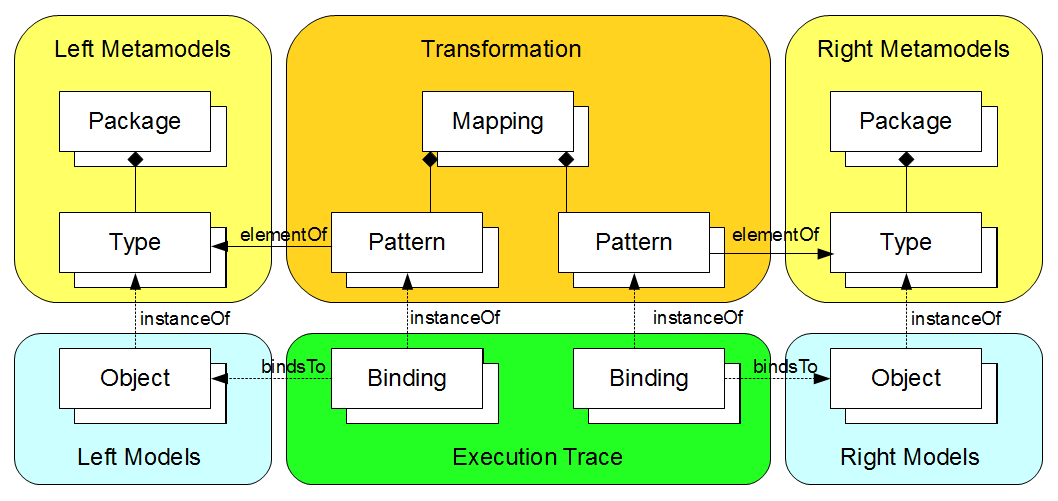
\includegraphics[width=0.45\textwidth]{TransformationAnatomy.png}
%	\caption{Transformation Anatomy.}
%	\label{fig:TransformationAnatomy}
%\end{figure}

QVT Core (QVTc) is a multi-directional, multi-input, multi-output declarative model transformation language. For simplicity, in the following description, we defer consideration of more than just a simple left to right creation until Section\ref{Future Work}. 
%The multi-directional capability allows a single QVTc transformation program to specify many model transformations, and to avoid the inconsistencies that may arise through writing independent programs for each direction and enforcement. QVTc supports the definition of \textit{check}, \textit{update} or \textit{create} transformations. 

A significant challenge for model transformation arises in specifying how the overlap of target Bindings is to be handled. A common solution provides specialized constructs to interrogate the execution trace and so allow the instantiation of one Pattern to interact with the instantiation of another. These specialized constructs are often rather obscure. QVTc is unusual in making the traceability model explicit; it is called the Middle model.

Comparison of Figure \ref{fig:QVTCoreAnatomy} with Figure \ref{fig:TransformationAnatomy} shows the distinctive Middle Metamodel. A QVTc transformation is therefore specified as a set of mappings with constraints defined in a domain for each left, right and middle model. Since the execution traceability must be explicitly defined, a \textit{Middle Model} (and metamodel) are used to define and instantiate the trace classes. It is important to note that it is the transformation author's responsibility to design the Middle metamodel.

%The complexity of the many relationships is managed by exploiting the metamodels, shown at the left and right hand sides of . These comprise packages and types to categorize the different kinds of objects in a model. The Transformation adds Mappings and Patterns to organize the different kinds of relationship to be satisfied.

\begin{figure}[h]
	\center
	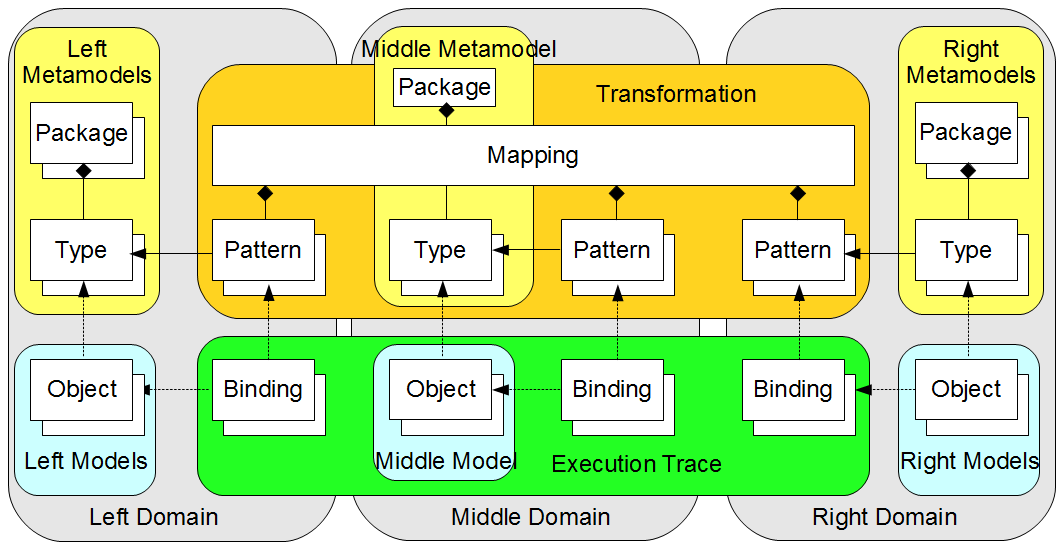
\includegraphics[width=0.45\textwidth]{QVTcore.png}
	\caption{QVT Core Anatomy.}
	\label{fig:QVTCoreAnatomy}
\end{figure}

The additional Middle model may be quite simple and the Middle Bindings may be free from overlap. This may significantly simplify the transformation exposition since with the aid of the intermediate, a direct N:M mapping from left-to-right may be expressed as a two-pass transformation comprising an N:1 left-to-middle pass and a 1:M middle-to-right pass. Any information that needs to be gleaned from the left can be cached in the middle model during left-to-middle pass so that it is readily available for use during the middle-to-right pass. Very complex transformations may specify additional passes that operate from Middle model to Middle model. QVTc supports reuse of mappings within a transformation by refinement, and reuse of transformations by inheritance.

The simpler semantics of QVTc  make a QVTc implementation of a declarative transformation more tractable. QVTc makes only small abstract syntax extensions to EMOF and OCL. A QVTc implementation is therefore an attractive intermediate implementation approach for QVTr, as suggested in the QVT specification.


%Figure \ref{fig:pattern} is an Object Diagram showing an example Pattern describing a parent-child match. The pattern involves two pattern variables \textit{theParent} and the \textit{theChild} each of which may be bound to a \textit{Node} object in a user model. The pattern imposes the additional constraint that the objects bound to \textit{theParent} and  \textit{theChild} variables must lie at each end of a \textit{parent}-\textit{children} Association. The \textit{theParent} lies at the composing (diamond) end of an optional (?) multiplicity.  The \textit{theChild} lies at the end of an arbitrary (*) multiplicity.

%\begin{figure}[h]
%	\centering
%	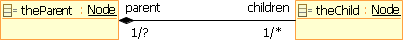
\includegraphics[width=0.45\textwidth]{pattern.png}
%	\caption{Example Parent-Child Pattern.}
%	\label{fig:pattern}
%\end{figure}

%When the transformation relationships are satisfied, the models have been partitioned into groups of objects and every object is a member of at least one group. Each group is identified by a Binding in which the Type of each object conforms to the Type of the Pattern element to which the object is bound. The interrelationships between the bound objects similarly conform to the interrelationships between the pattern elements. For the example pattern, each Binding comprises a pair of \textit{Node}s one bound to \textit{theParent} and the other bound to \textit{theChild}. A Binding exists for every possible pair of \textit{Node} objects that match the Pattern. The transformation between the Bindings is defined by Mappings, each of which defines the interrelationships between one left Pattern and one right Pattern.

%The foregoing principles are common to many declarative and some imperative transformation languages. It is in the way in which mappings are structured that transformation languages vary.

%\subsection{Traceability and the Middle Model}
%A significant challenge for model transformation arises in specifying how the overlap of output Bindings is to be handled. A common solution provides specialized constructs to interrogate the execution trace and so allow the instantiation of one Pattern to interact with the instantiation of another. These specialized constructs are often rather obscure. QVTc is unusual in making the traceability model explicit; it is called the Middle model. Figure \ref{fig:QVTCoreAnatomy} shows how for QVTc there are three Domains, Left, Middle and Right, each of which comprises Models and Metamodels. Associated with each Domain are the Bindings and Patterns.

%\begin{figure}[h]
%	\centering
%	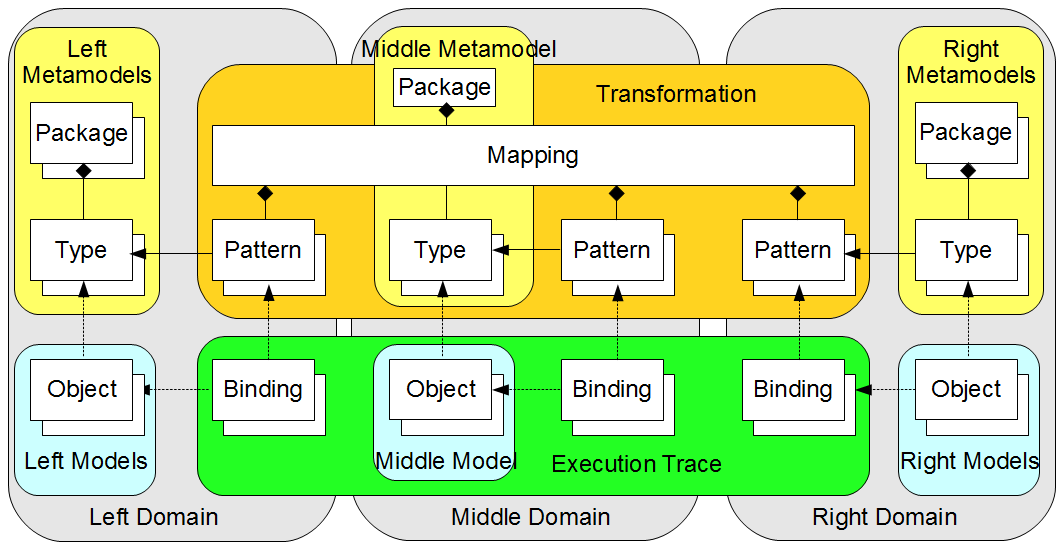
\includegraphics[width=0.45\textwidth]{QVTcore.png}
%	\caption{QVT Core Anatomy.}
%	\label{fig:QVTCoreAnatomy}
%\end{figure}



%The Middle model of course conforms to its metamodel and, for QVTc, it is the transformation author's responsibility to design the Middle metamodel so that overlaps can be resolved and information cached. %[The more powerful QVTr language, when implemented by a QVTc engine, requires the Middle metamodel to be synthesized as part of the QVTr to QVTc program to program transformation.]

%\subsection{Intra-Mapping Semantics}

Within a Mapping, the QVTc semantics are simple; each Domain comprises a GuardPattern and a BottomPattern. The GuardPattern is responsible for the matching, and the BottomPattern for the model mutation. 

\begin{figure}[h]
	\centering
	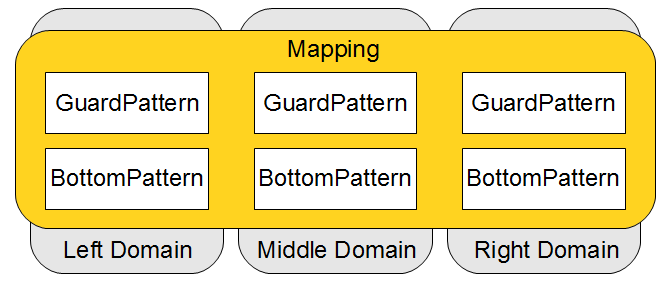
\includegraphics[width=0.45\textwidth]{QVTcoreAreas.png}
	\caption{QVT Core Areas.}
	\label{fig:QVTCoreAreas}
\end{figure}

The two-dimensional layout shown in Figure \ref{fig:QVTCoreAreas} is difficult to achieve in a text file and so the concrete syntax is

{\scriptsize \begin{verbatim}
map mapping-name in tx-name {
  left  ( left-guard-pattern-variables
        | left-guard-pattern-constraints )
        { left-bottom-pattern-variables
        | left-bottom-pattern-constraints }
  right ( right-guard-pattern-variables
        | right-guard-pattern-constraints )
        { right-bottom-pattern-variables
        | right-bottom-pattern-constraints }
  where ( middle-guard-pattern-variables
         | middle-guard-pattern-constraints )
        { middle-bottom-pattern-variables
        | middle-bottom-pattern-constraints }
}
\end{verbatim}}

Let us consider as complex an example of a bidirectional transformation as space permits; transformation of colored Node trees. The trees demonstrate recursive hierarchy and edges. The alternate color representations demonstrate attributes; HSV (hue, saturation, value) on the left, HLS (hue, lightness, saturation) on the right and RGB (red, green, blue) as a middle intermediate. Figure \ref{fig:TreeMM} shows the three metamodels with the additional traceability references from middle metamodel to the external metamodels.  Listing \ref{lsting:QVTcExample} presents the QVTc transformation for this example.

\begin{figure}[hb]
	\centering
	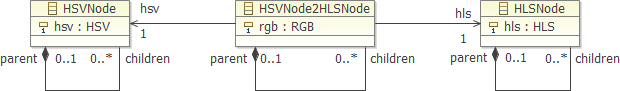
\includegraphics[width=0.45\textwidth]{Metamodels.png}
	\caption{Simple Tree metamodels; Left(HSV), Middle(RGB), Right(HLS).}
	\label{fig:TreeMM}
\end{figure}

\input{qvtc.lst}

Lines 2-5 express the \texttt{transform\-ation} declaration including our proposal of using an unnamed \textit{TypedModel} for the middle model. The bodies of the the color converter queries (lines 8-11) are omitted for space reasons.

Lines 13 to 25 provide the \textit{Node2Node} mapping, without any guard variables or constraints; the mapping is therefore unbound. Each domain realizes a \textit{Node}, and so requires that where that node exists in a source domain, the corresponding nodes are created or updated in the middle and target domains. Lines 21 to 24 initialize the middle node from whichever of \textit{hsv} or \textit{hls} is the source.

Lines 27 to 34 refine the \textit{Node2Node} mapping to enforce consistency at the root so that all root nodes have no parent. Lines 36 to 43 refine the \textit{Node2Node} mapping to enforce consistency of parent-child relationships. The guard pattern introduces an additional parent node variable for each domain and requires that this is indeed the parent of each node inherited from \textit{Node2Node}. For the source domain, the parent-child relationship is interpreted as a guard, whereas for the middle and target domains, the parent-child relationship is enforced.

The foregoing quick summaries demonstrate how symmetrical definition of multi-directional transformations is supported by the combination of the pattern variable declarations, some of which can be realized while others must exist, and by the assignments of OCL queries to properties. Some declarations are distinct for each direction, while others adopt distinct predicate or assignment semantics according to the transformation direction.

% In each domain we are interested in two elements (the parent and the child), so we need two pattern variables to capture the two parts of a Binding. These variable are constrained, firstly by their type, secondly by an explicit constraint that the two nodes have the same color and finally by an explicit constraints that one fulfills the relation of being the parent of the other. A naive transformation tool may just iterate each variable over each model element to identify each candidate binding and then prune those that fail to satisfy all constraints. A slightly more intelligent tool may iterate only over the model elements that conform to the required type. For this trivial example all model elements are of the same type so a type check achieves little. For more realistic metamodels the basic type constraint should significantly reduce the mantissa of an exponential computation cost. A much more intelligent tool should exploit the metamodel relationships so that at most the first pattern variable involves a full model search; subsequent variables can be searched for locally. In our example, after choosing a parent candidate, only its children need consideration. Careful use of the metamodel to plan search strategies can reduce the naive exponential complexity to something much closer to linear for many practical problems.

% Returning to the QVTc exposition. The GuardPattern orchestrates the search, so in the GuardPattern we declare the two pattern variables with their constraining types and provide the additional matching color constraint. Once the GuardPattern has been satisfied, the BottomPattern provides the copy of the selected child from left to right.

% Our example loses information and so cannot be executed in reverse. However we can still examine the example to understand the symmetries that QVTc provides. In the forward direction, an assignment defines the valid right hand output from left inputs. Conversely for a reverse transformation the forward assignment acts as a predicate rejecting candidate right hand elements that are inconsistent with the forward transformation. For example on Listing \ref{lsting:QVTcExample} if the transformation was executed in the direction of the \texttt{subTree} model, the predicate in line 21 will cause the \textit{color} attribute of \textit{\textbf{cT}} to be set to the value of the \textit{color} attribute of \textit{\textbf{pT}}. If we executed the transformation in reverse (i.e. in the direction of \texttt{coloredTree}) then the predicate in line 21 will act as a constraint evaluating that both elements have the same \textit{color}.

%\subsection{Inter-Mapping Semantics}

%A single mapping is of limited utility. Practical transformations require many mappings and an ability to share context between mappings. Consider a mapping from a hierarchical metamodel such as UML. A high level mapping may transform packages, and the transformed package is then needed as context for a mapping involving classes. QVTc supports independent mappings by declaring each as a top level mapping as in Listing \ref{lsting:QVTcExample}. Shared context is supported by declaring the dependent mappings as nested within the mapping whose bindings the nested mapping shares as in Listing \ref{lsting:QVTiExample}.

%\subsubsection*{Execution Modes}

%A multi-directional transformation does not have unambiguous inputs or outputs and so a QVTc transformation is specified between TypedModels. In practice only one direction will be of interest at any one time and so once the invocation identifies which TypedModels are inputs and which are outputs, a practical QVTc tool may optimize away the redundant declarations for unwanted directions. Since all transformations are not reversible, QVTc allows the programmer to restrict particular Domains to input or output in order to specify \textit{check} or \textit{create} functionality, by using the \texttt{check} or \texttt{enforce} keywords.

%\textit{Update} functionality can be achieved by specifying the same model as the input and output model. For this use case, the declarative QVTc exposition enables the QVTc tooling to ensure that the update occurs in a coherent fashion so that all input locations are read before any co-located output locations are written.

%\subsection{Program-to-program Transformations}
%\subsubsection*{QVTc to QVTu}
%A single direction and mode (create or update) must be selected. Based on this selection the transformation is modified to remove bi-directionality making the input model read-only. 
%\subsubsection*{QVTu to QVTm}
%Two major activities take place: elimination of rule inheritance and partition rules into left-to-middle, middle-to-middle and middle-to-right. Elimination of rule inheritance increases verbosity but reduces semantic complexity. Partition of mappings facilitates scheduling.
%\subsubsection*{QVTm to QVTi}
%Nested mappings are replaced by mapping calls (new in QVTi) and produce the final imperative scheduling.